\documentclass[11pt, letterpaper]{article}
\usepackage[utf8]{inputenc}
\usepackage{graphicx}
\usepackage{indentfirst}
\usepackage{float}
\setlength{\parindent}{5ex}


\usepackage{geometry}
\usepackage{booktabs}
 \geometry{
 letterpaper,
 left=1.2in,
 top=1in,
 right=1.2in,
 bottom=1.1in,
 }

\begin{document}

\begin{titlepage}
    \begin{center}
        \vspace*{1cm}

        \Huge
        \textbf{PID Controller Manual}

        \vspace{0.5cm}
        \LARGE

        \vspace{1.5cm}

        \textbf{Alexander Fogal}

        \vspace{7.8cm}

        \Large
        For Professor Jim Martin\\
        University of Waterloo\\
        August 2021

    \end{center}
\end{titlepage}

\tableofcontents

\newpage

\section{Introduction}
Welcome! This is an instruction manual for the PID Control system I worked on for Professor Jim Martin, it was designed to replace the previous system, and this manual is meant to replace the manual that came with that system. Because of this, significant portions of information were carried over more or less verbatim.

\subsection{Purpose of this Manual}
This document is meant to offer all the information required to use and understand this PID Control system. If any problems arise in the system, or any modifications need to be made, this document is meant to be a one stop shop for information.

The operation section will detail daily use with the controller. It will detail hooking up the controller, the onboard interface, and the remote control interface. The hardware section will detail the PCB, microcontroller, and each component. The software section will detail how various parts of the code work, including internet connectivity, the MQTT protocol, how the persistent settings work, initialization and the main loop, integral windup control, and error control and the "Current Error" message. The building, debugging, and modification section will contain information about programming the controller, acquiring data, the PCB and schematic, and other debugging information. Finally, there will be an appendix about control theory and the control theoretical justification for this system.

Hopefully the information you need will be contained in these pages!

\subsection{Purpose of the Controller}
This controller was originally designed to manage a rubidium vapour cell heater and current source for experiments on Rydberg Atoms. The temperature of the vapour in the cell was required to be maintained above ambient temperatures, up to $100^{\circ} C$ depending on the experiment. Such a system is required due to background fluctuations and drift in ambient temperature. The long time constants involved make an analogue circuit impractical$^{[1]}$, hence a digital system was used.

Despite the specific motivation, this PID controller is generic and customizable such that it can be used to manage any suitable process. For example, it could be potentially used to control a vacuum chamber bake-out oven.


\section{Operation}
This section will detail day to day operation of the controller, including initial setup.

\subsection{Connecting the Device}
The controller has three BNC and one ethernet connector on it (Version 1 boards also will have an exposed micro usb, which is for programming the microcontroller and power). The ethernet will carry power via Power over Ethernet (PoE), which will power the unit. The three BNC connectors are split up by input and output: there is one BNC output that carries the control signal to the current source (labelled CurrOut BNC on the PCB), and there are two BNC inputs, one that carries the thermistor signal (ThermIn BNC on the PCB) and one that carries the current monitor signal (CurrIn BNC on the PCB).

\begin{figure}[H]
    \centering
    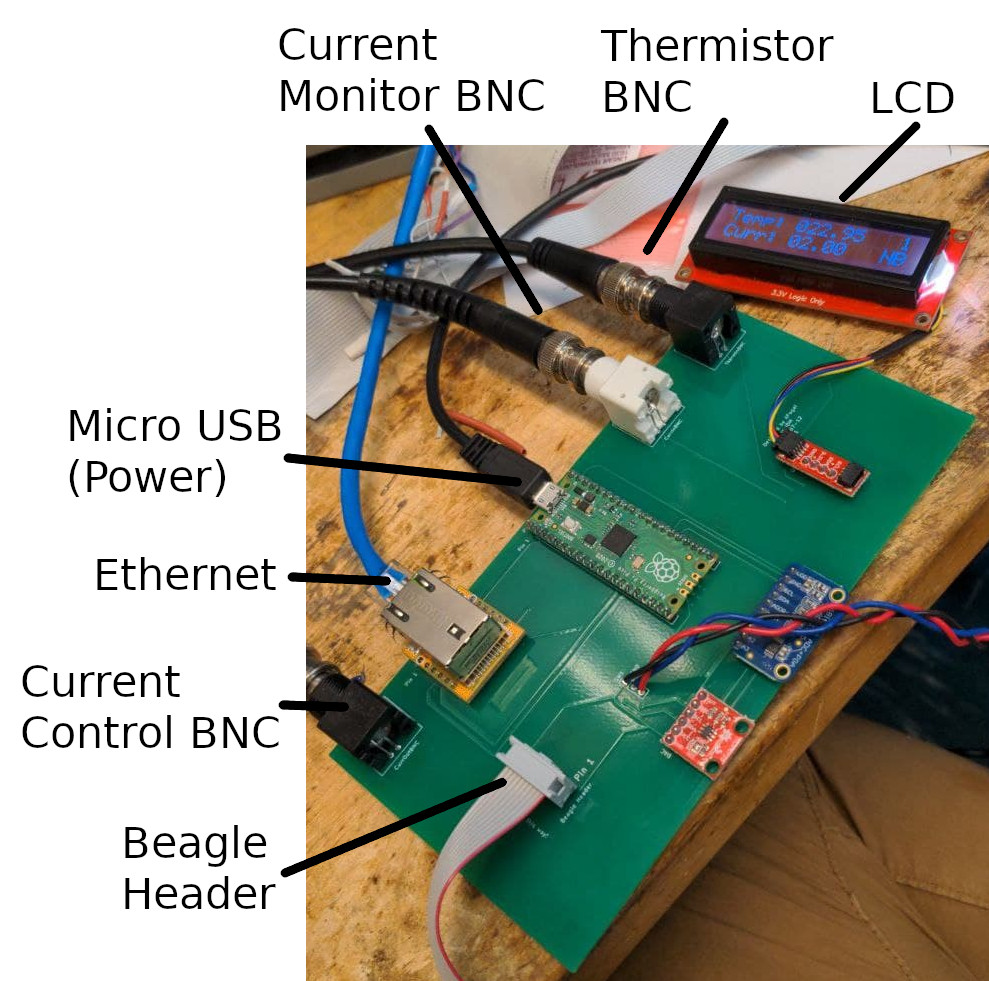
\includegraphics[width=15cm]{controllerConnections.jpg}
    \caption{ Connectors on the back of the Controller }
    \label{fig:controllerConnections}
\end{figure}

\begin{figure}[H]
    \centering
    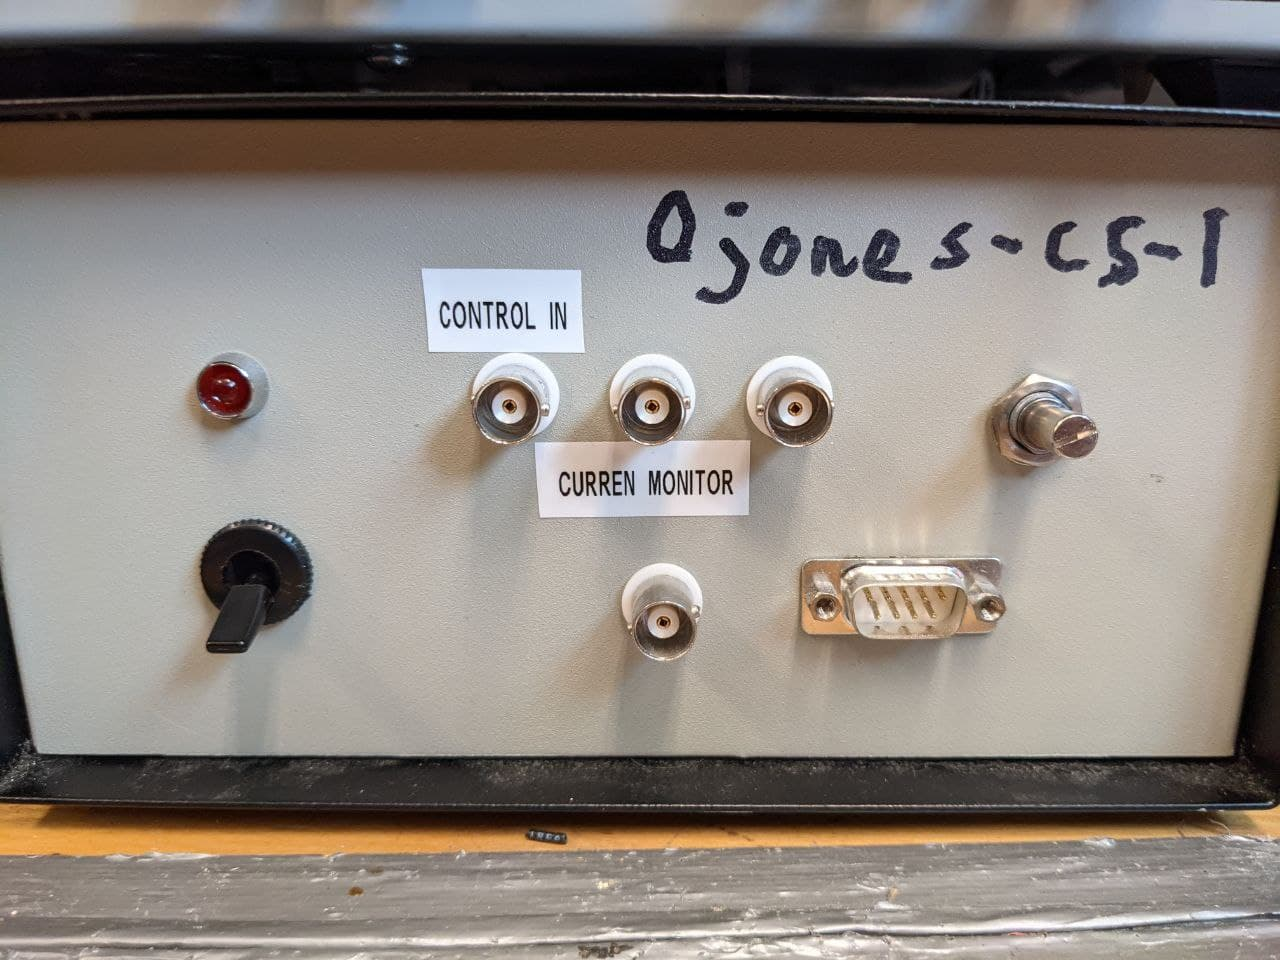
\includegraphics[width=15cm]{currentSourceConnections.jpg}
    \caption{ Connectors on the front of the current source }
    \label{fig:currentSourceConnections}
\end{figure}


The current source has several connections on the front: "Control In" is a 0-5V control signal, with 5V being the max current; "Curren [sic] Monitor" (the top BNC) is, similarly, a 0-5V signal, this time for reading back to make sure the current matches the expectation; the two unlabelled BNCs are, I belive, feedback and measurement thermistor signal lines, but I have not tested this directly; finally, the D-SUB is to connect to the Rubidium cell, and it has the following pinout:

\begin{table}[H]
    \centering
    \begin{tabular}{ll}
        \toprule
        \textbf{Pins} & \textbf{Function} \\
        \midrule
        1,2 & Heater Gnd \\
        3,4 & Main Heater +ve \\
        5,6 & Secondary Heater +ve \\
        7 & Measurement Thermistor +ve \\
        8 & Feedback Thermistor +ve \\
        9 &  Thermistor Gnd \\
        \bottomrule
    \end{tabular}
    \caption{Pinout of Current Source D-SUB}
    \label{tab:sourcePinout}
\end{table}

The D-SUB connects to the Rubidium vapour cell heater, but it is also possible to use external thermistors, which can be calibrated via code (see the last section).

\subsubsection{Test Cell Setup}

The test cell setup differs from the experiment setup slightly. The test cell is a large aluminium block with a heater and several different measurement devices. These thermal measurement devices are connected to a small box with an XLR connector and several BNCs. The XLR provides power via the following pinout:

\begin{figure}[H]
    \centering
    \includegraphics[width=6cm]{XLRPinout.png}
    \caption{ XLR power pinout convention (used in lab only!!) }
    \label{fig:XLRPinout}
\end{figure}

Each BNC connector corresponds to a different measurement device, I used the LM355 for simplicity, as it is internally calibrated to have a voltage equal to the temperature divided by 100. The most accurate measurement comes from the yellow plug, which is a thermistor, but that requires external measurement circuitry.

So, to hook up the controller to the test cell setup, connect the current control and current monitor BNCs to the current source as normal, connect the custom D-SUB cable to the current source, and wire the black and red wires to the black and red heater terminals on the back of the box. I used an external power supply set to +15V and -15V connected to an XLR plug to power the box.

\begin{figure}[H]
    \centering
    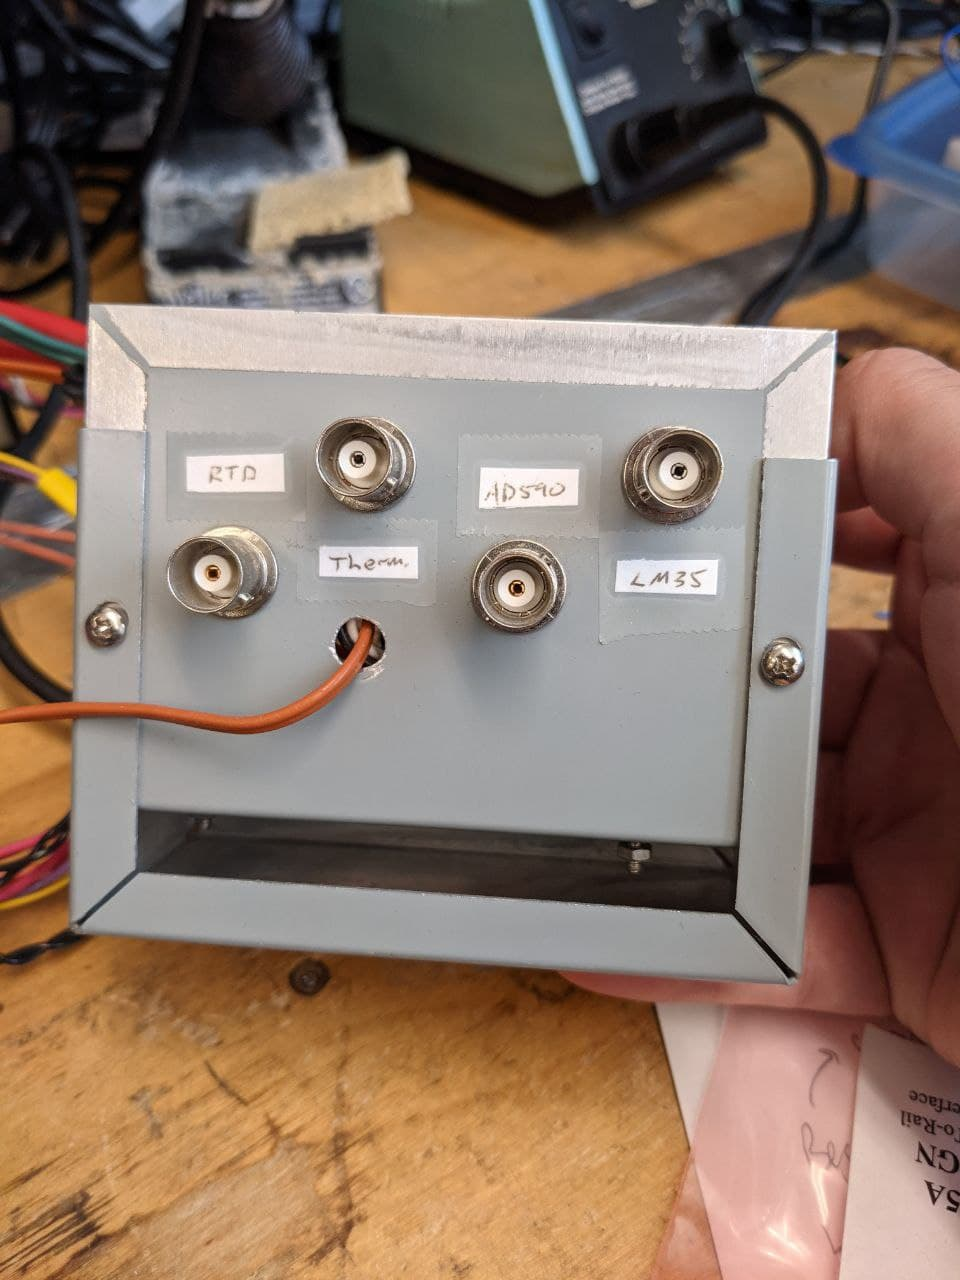
\includegraphics[width=10cm]{testCellBoxFront.jpg}
    \caption{ Test Cell Box Front }
    \label{fig:testCellBoxFront}
\end{figure}

\begin{figure}[H]
    \centering
    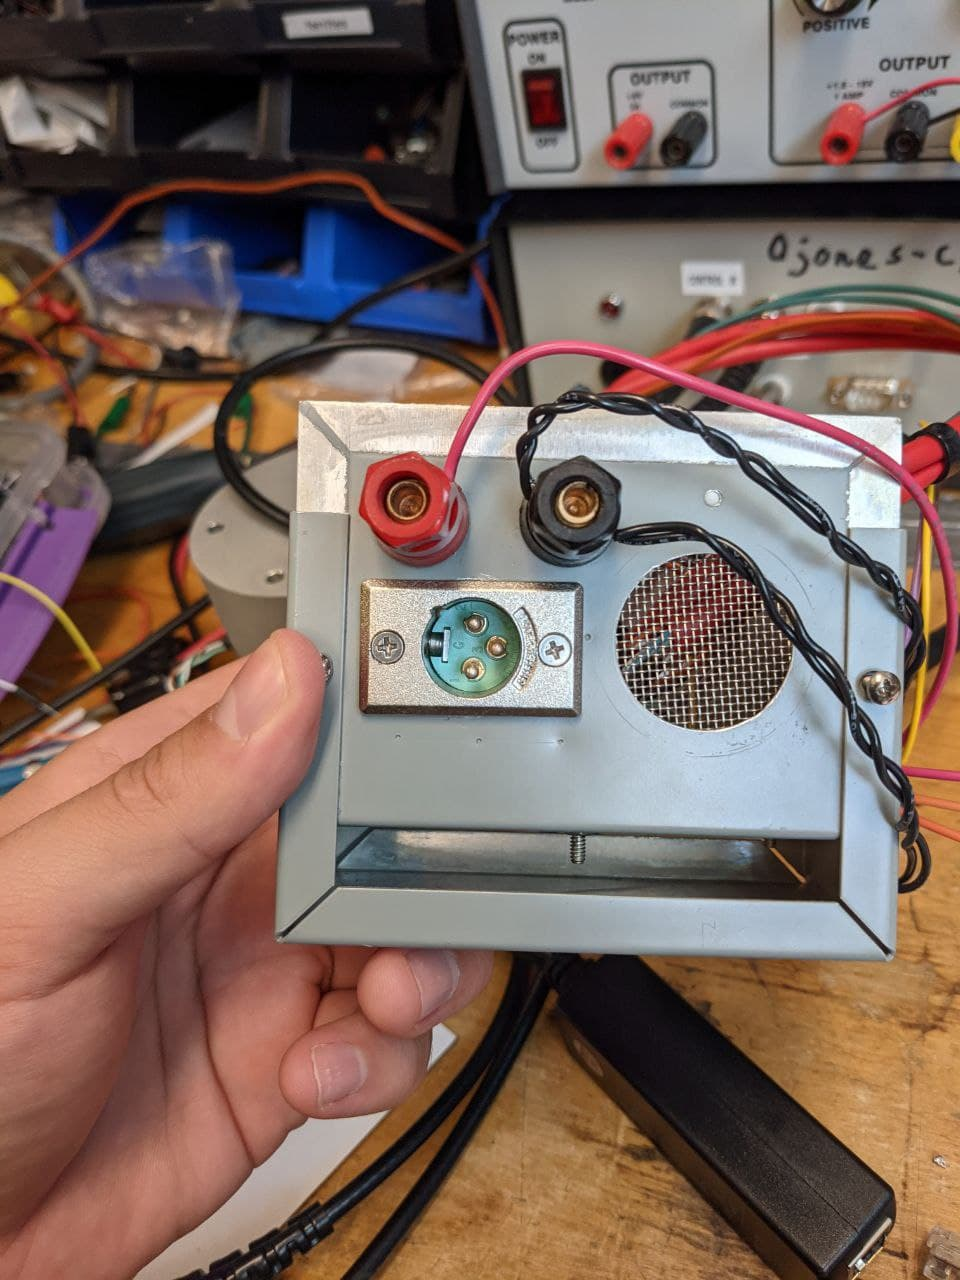
\includegraphics[width=10cm]{testCellBoxBack.jpg}
    \caption{ Test Cell Box Back }
    \label{fig:testCellBoxBack}
\end{figure}

\begin{figure}[H]
    \centering
    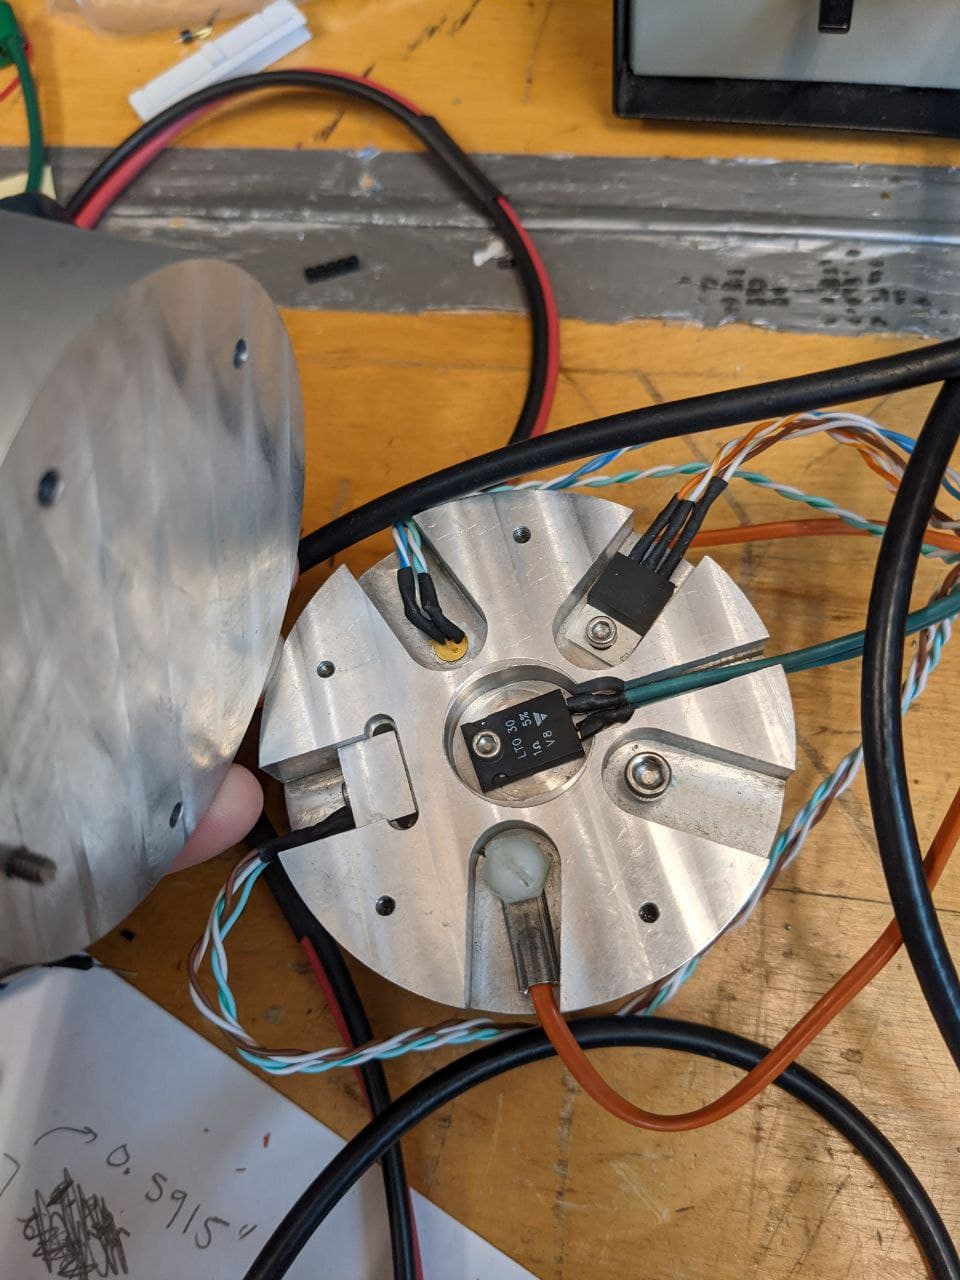
\includegraphics[width=10cm]{testCellSetup.jpg}
    \caption{ Test Cell }
    \label{fig:testCellSetup}
\end{figure}

\subsection{Controller Interface}

The interface on the actual controller is quite straight forward:

\begin{figure}[H]
    \centering
    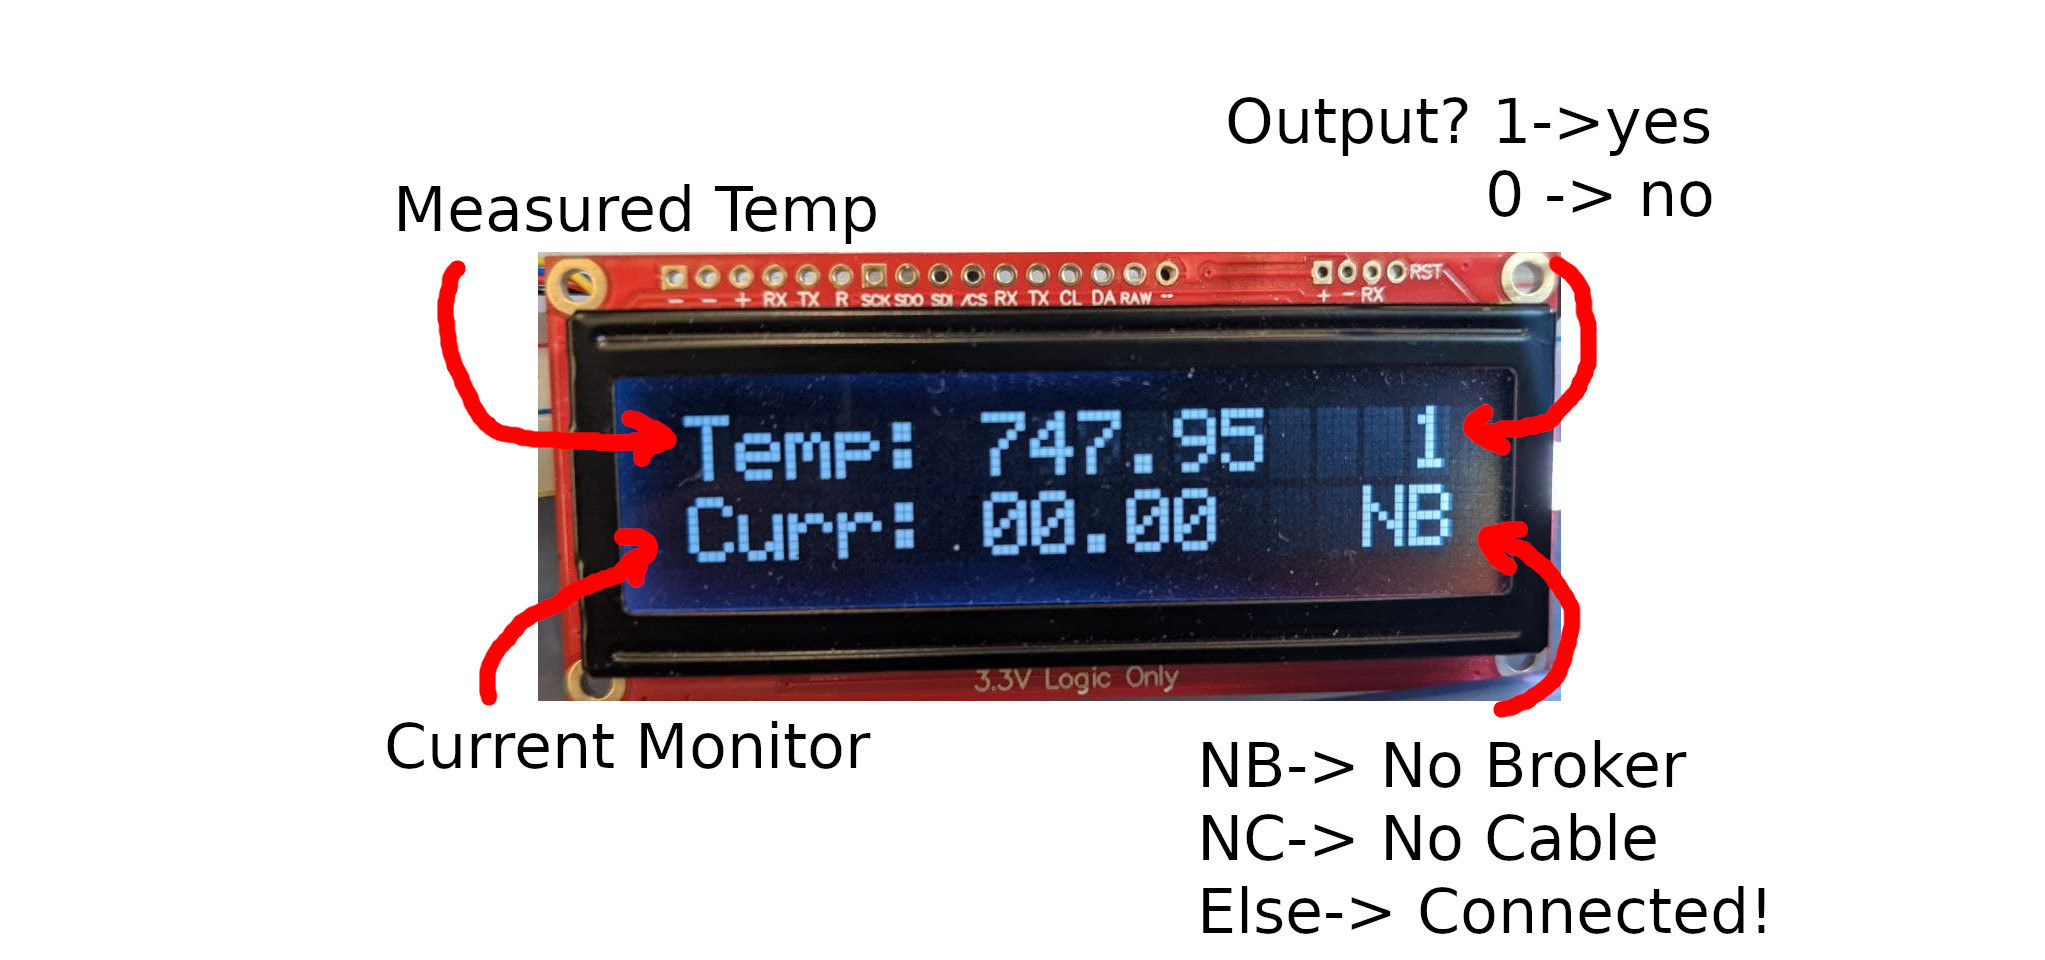
\includegraphics[width=11cm]{screen.jpg}
    \caption{ Controller UI Layout }
    \label{fig:screen}
\end{figure}

All parameters are changed via the remote interface.

\subsection{Remote Interface}

The remote interface is where all the magic occurs! It looks like this:

\begin{figure}[H]
    \centering
    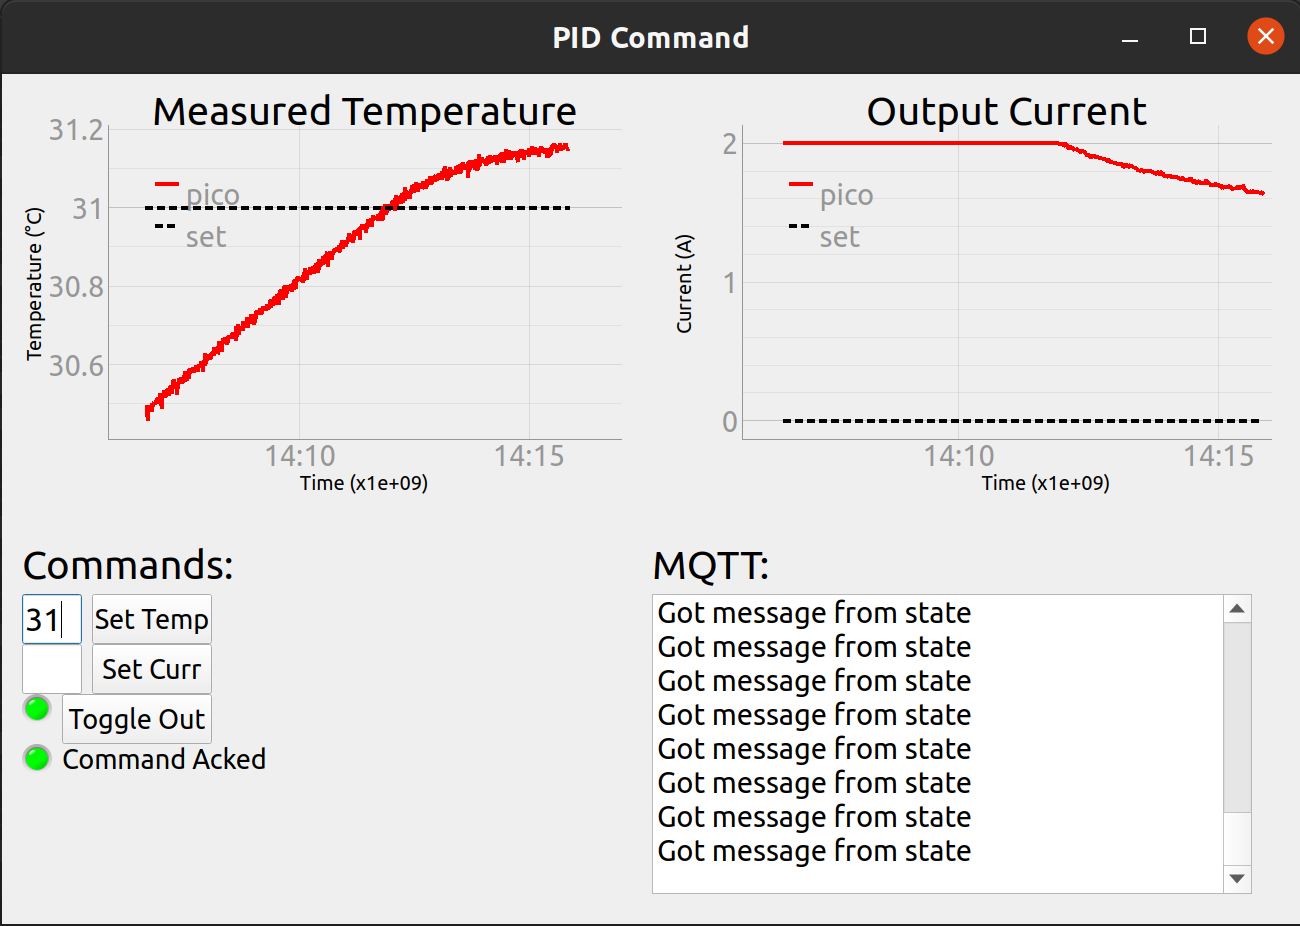
\includegraphics[width=12cm]{command_ui.png}
    \caption{ Remote Command UI }
    \label{fig:command_ui}
\end{figure}

The functions are all quite straight forward: to change the set temperature, type in a number and press the "Set Temp" button (note that no checking is done on the number you put in, if it fails to convert there will be a message in the box); to change the set current, type a number in the box and push the "Set Curr" button (note that there is no checking on this either, please only enter values 0-2 or whatever the controller is configured for); in order to stop the current outputting, click "Toggle Out", the indicator will be green when it is outputting, and red when it is not. Every time a command is performed, the "Command Acked" indicator will turn red, and it will turn green again if the controller successfully performs the command (and internet is working).

There are also graphs of the temperature measured and current being outputted for convenience.

\section{Hardware}

This section will detail each hardware component of the controller.

\subsection{Raspberry Pi Pico}

The Raspberry Pi Pico is the brains of the operation: the microcontroller unit (MCU). It runs the adafruit distribution "CircuitPython" as well as related adafruit libraries. It is well suited to this task due to the ease of use in programming (you can plug it in and be programmed via usb), $I^{2}C$ functionality, low cost, computing power, and wide variety of libraries for programming. Additionally, we expect that it will be produced for years to come in case replacements are required.

Digikey part number: SC0915

\subsubsection{$I^2 C$}

The MCU controls the DAC, ADC, and LCD via the $I^2 C$ protocol. This was done because it requires only two connections (in addition to power), and is relatively easy to debug using a tool like the Beagle I2C spy device. Note that the ethernet is {\it not} controlled via $I^2 C$, but is rather controlled using SPI. Note that both SPI and $I^2 C$ are available on the header pins on the PCB.

Note that $I^2 C$ lines are "open drain", which means they are connected to VCC (3.3V in this case) via pullup resistors. The two $I^2 C$ lines are SDA (data) and SCL (clock). The MCU acts as the "master" device, and must initiate any exchange. Note also that long $I^2 C$ lines can cause excessive capacitance, which may cause a communication breakdown. Furthermore, it is possible to hard-lock the $I^2 C$ bus if the MCU resets at the wrong moment during communication. In this case, a power cycle is required.

\subsection{DAC}

This DAC is responsible for sending the current control signal to the current source. The DAC has 12 bit resolution and is wired to produce a signal from 0-5V, at 12bits this is (ideally) steps of 0.0012V. Another advantage of this DAC board is that the actual DAC chip is quite common (MCP4725), and adafruit has a library to control it easily. The maximum current this chip is rated for is 24mA, which is sufficient to signal the current source.

Digikey part number: BOB-12918

\subsection{ADC}

The ADC is responsible for reading the thermistor and current monitor signals. The ADC has 4x16 bit single ended channels, or 2x16 bit differential channels. The ADC is wired up for differential measurements in this case, with the signals being compared to "Analogue Ground", which is connected to the DAC ground and the BNC shields. This ADC is capable of measuring 0-5V signals, and has a programmable gain factor (currently set to 1). This ADC is capable of sampling at 860 Hz, which is more than sufficient for this application.

Digikey part number: 1085

\subsection{Ethernet}

We desired to have this controller be controlled via the internet, while not sacrificing speed as one might by using a fully fledged Raspberry Pi SoC. Therefore, we added a peripheral ethernet jack. This ethernet jack/chip combo board allows the MCU to connect to remote sources via the SPI protocol. To control this, another adafruit library was used. Note that this chip is technically capable of engaging with DNS, but it is currently setup only for a static IP, which may need to be changed for future applications.

Digikey part number: WIZ850IO

\subsection{LCD}

The LCD is a 2 line by 16 character display running on the open source SerLCD toolkit. The LCD has contrast and brightness control if desired. The LCD is only compatible with 3.3V $I^2 C$ logic, and can only be powered from 3.3V as well. This LCD was selected due to having the SparkFun QWIIC cable, which makes it easy to move and test.

\subsection{PCB and Box}

This PCB was designed in-house using KiCAD, the files are available for it on Github. This was done partly as a learning experience, partly for robustness, and partly for generality. The PCB is meant to be mounted to a box via the BNCs. The PCB also eliminates any errors that could come from a misconnection or miswiring of the components.

\subsubsection{Version 1}

Version 1 of the PCB was intended to be powered directly from the micro USB on the pico, which was changed to PoE for version 3. Version 1 had two major faults: the ADC differential channels were wired backwards (so all positive voltages read negative), and the digital ground was not connected to the MCU. The first of the two faults was taken care of in the code, and the second required a wire to be soldered between any of the ADC, DAC, or pin header grounds to either the MCU or QWIIC adapter ground.

\subsubsection{Version 2 and 3}

Version 2 of the PCB fixed the above faults, and was never produced. Version 3 incorporated those fixes and the board was rearranged to make it more suitable for PoE and a single ethernet jack on the box to be used. As of the time of writing, version 3 has not been produced yet either.

\subsubsection{Box}

The Box we chose was a Hammond Mfg. 1590D box, due to it's wide availability and size being approximately correct for the PCB as it was designed. A drawing of where the holes should be is available on Github. The drawing was done in a free trial of QCAD. There is only one version of the box, which corresponds to PCB V3.

Digikey part number: 1590DGY

\section{Software}
This section will cover the details of the software used in the controller. For a brief overview, the major sections of the code are as follows: first there are imports; then there are constants and variable definitions and pin setup; then there is the default settings dictionary and an attempt to load old settings; then there is PID variable definitions; then there is a function definition block; then the major setup block including $I^2 C$, DAC, ADC, ethernet, and MQTT setup and connectivity; then some loop variable initialization; and finally the main loop. Please refer to the following sections for a more in depth exploration.

\subsection{Internet}
Internet connectivity is achieved through the adafruit \verb|WIZNET5K| library, which manages the SPI bus, and really, all of the heavy lifting. It is technically possible to use DHCP for dynamic IP allocation, but at the time of writing there was a bug in the library for this feature, and really, a static IP is better for this application anyways.

First, the SPI pins are defined, and the various internet related parameters are defined, eg MAC address, IP address, Gateway and Subnet addresses, and the DNS server. These parameters may need to be modified to suit whatever network this controller is deployed on. Next, the SPI bus is defined, which is handled by the adafruit \verb|busio| library. The ethernet controller is initialized via an initial reset, and then the library is initialized, and the configuration parameters are set. The \verb|socket| library is also initialized to use the newly defined ethernet connection. At this point, the rest of the connectivity is handled via MQTT and the relevant adafruit library, although low level socket calls can be made now as well.

\subsection{MQTT}
MQTT stands for "Message Queuing Telemetry Transport", and it is the protocol used for communication between the controller and the remote computer. It was chosen due to the very small amount of data transmitted, and the relative ease of use that comes with preexisting adafruit libraries (as opposed to, say, making low level socket calls and dealing directly with TCP). Additionally, the asymmetric nature of MQTT made the most sense for this application. From the MQTT commitee website:

\begin{figure}[H]
    \centering
    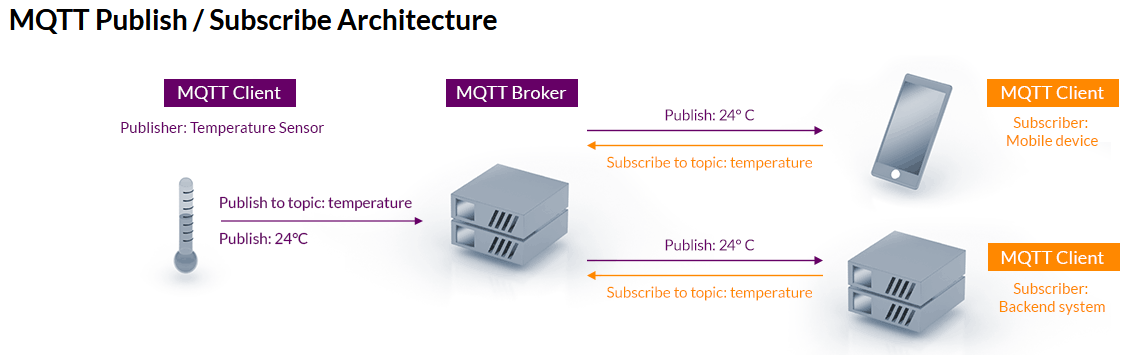
\includegraphics[width=16cm]{mqttArch.png}
    \caption{ The MQTT paradigm }
    \label{fig:testCellSetup}
\end{figure}

This asymmetry is not strict though, a client can also be a publisher, and a publisher can also be a client. In this way, the Pico publishes measurements and subscribes to commands, the remote computer publishes commands, and subscribes to measurements. The use of a broker in this application allows any published messages to be rebroadcasted to a device when it comes back online, the relevant terminology for that is Quality of Service Level (QoS). In our particular application, commands and measurements are broadcasted as json packets, which allows convenient labelled and avoids confusion down the road.

To pick up where we left off in the previous section, after establishing internet connectivity, the adafruit \verb|mini_mqtt| library is used to establish an MQTT context. The relevant interface and socket are passed to the library, and the initialization is performed. Additionally, a function is provided to the instance to be called when messages are received. At this point, the actual connection is attempted (the \verb|clean_session=False| parameter allows faster reconnections and rebroadcasting of any missed messages), and a subscription to the commands feed is established with QoS level 1 (rebroadcasting). If successful, boolean variables are set to define what parts succeeded/failed. 

In the main loop, whenever a suitable amount of time has elapsed (defined by \verb|defaultSettings['mqttDelay']| ), the client asks for any new messages from the broker with the shortest timeout possible. Then, the client publishes the current state. There is some error handling here to attempt reconnection should the internet fail in some way.

If there are any new messages, the \verb|do_command| function is called, which parses the json and performs the appropriate action, and gives a suitable response.

\subsection{Persistent Settings}
The controller is capable of having persistent settings, that is, if it were to lose power, it would boot up in the last configuration. This comes with one small caveat, being that if the MCU can write to flash, a connected computer cannot. This is the purpose of the switch on the controller, one position is to enable programming the MCU, and the other position enables persistent settings. In order to save the settings, the \verb|defaultSettings| dictionary is saved as a json file.

One must be careful of these persistent settings, as the networking configuration is a part of them! If one needs to change the IP or something, it may be better to simply delete the persistent settings file and change the value in the code file.

\subsection{Initialization and Main Loop}
There is a lot of initialization so buckle up! First is the I2C bus, which is passed the SCL and SDA pins as well as a frequency. The frequency is not super important, although higher frequencies often mean difficulties in communication when there are more devices and longer wires involved. Then, the lcd is initialized using a generic adafruit library and a string is printed to it. 

The next initialization is the DAC, for which there is an adafruit library that handles the hard stuff. This is the same story for the ADC. It is worth noting that here the differential pairs are defined, and they cannot be arbitrary pairs or in an arbitrary order. The purpose of using differential pairs is to have a separate analogue ground, which is defined by the BNC shields. This analogue ground is used for the DAC as well. The continuous mode on the ADC is unusable with multiple ADCs in use, so we keep it in the default (single) mode, which causes the ADC to hang on read until there is a fresh value. For this reason, the max sampling rate is used as well.

The main loop involves 4 main parts. Each part runs after a certain amount of time has elapsed since the last time it was run. Please be careful with the timing, the time is handled in nanoseconds. Fortunately, one of the upsides of using python on a MCU is that it supports arbitrarily large integers, so the time will never overflow! The first portion is the MQTT send and receive block, which receives any commands and sends the current state. The second block is the MQTT reconnect block. The third block is the main PID loop, which entails:

\begin{enumerate}
    \item Reading the thermistor and current voltages and convert to temperature
    \item Save current error and time, exponentially weight recent errors (and trim if there are too many being saved)
    \item Compute the P, I, and D (currently disabled) signals, clamping the I signal if it is too large, and combining
    \item Detect if measured current does not match expectation, shut down if this lasts too long
    \item Write the new signal to the DAC
    \item Keep track of sampled signals to report an average if desired.
\end{enumerate}

The final block is for updating the LCD (otherwise the info on it would be constantly changing and very difficult to read). Be very careful not to go over the edge of the LCD in a single write action, it causes the LCD to soft lock, which hard locks the I2C bus, requiring a power cycle. There are some alternate readouts for the LCD available in the code to assist debugging including a voltmeter. 

\subsection{Integral Windup and Clamping}
There exists a phenomenon in PID control called {\it Integral Windup}, which refers to when the integral term integrates the error abnormally large, usually due to the process becoming disconnected in some way. There are two ways this is handled by the controller right now. The first way is by limiting the magnitude of the integral term, and the second way is by comparing the expected current to the measured current, and stopping if they do not match over a long enough period. This produces the "Current Error!" message on the LCD. This message can be cleared by toggling the output off and on again. Usually, the cause of the current error dialogue is disconnecting either the current output or current input BNCs.

\section{Building, Debugging, and Modification}
This section will briefly cover making additions or modifications to the hardware of the controller.

\subsection{Adding/Calibrating Thermistors}
In order to add or calibrate thermistors, one needs the resistance at $25^{\circ}$C and the thermistor beta value. These will need to be updated in the \verb|defaultSettings| dictionary, and if persistent settings are used, then it should be updated there too.

\subsection{Programming and Debugging}
Programming is, thankfully, really quite simple. Make sure the switch is set such that it allows writing to the flash (the red and blue wires should be connected), and then connect the micro usb on the MCU to a computer. The MCU will show up as a storage device, and you can edit \verb|code.py| right then and there using your preferred editor. I used \verb|thonny| (not the one available in the Ubuntu repos, that one is out of date, download the fresh one directly from their website), which after some trivial setup, allows running code and REPL directly on the MCU itself. This is useful for debugging, because you can then actually see errors when they occur, read outputs directly, and more. 

\subsection{Acquiring Data}
Acquiring data has also been designed to be easy. The all of the data is sent out to the remote interface, and is simply logged and saved there according to when the remote interface was started. This comes with the somewhat obvious downside that the remote interface should be running for the full data collection period, although intermittent internet connection should not pose difficulties due to the MQTT QoS level. 

Should one desire to have more frequently sampled data points, one can simply decrease the timeout before sending another message, i.e., lower \verb|defaultSettings['mqttDelay']| to the desired period of data collection.

\subsection{PCB and Schematic}
The PCB and schematic were designed in KiCAD. There is not really an easy way to make modifications without learning the entirety of how to use KiCAD and how PCBs are designed. Very simply, there are two layers to the PCB: front and back. Traces can be put on either layer, and if they touch on the same layer then they are connected. Traces can be connected between layers by vias. The pin spacing is 0.01" or 2.54mm (standard breadboard spacing). 



\end{document}